\documentclass[a4paper, 12pt]{article}

% ==================== Packages ====================
\usepackage{geometry}            % Page layout
    \geometry{left=2.5cm, right=2.5cm, top=2.5cm, bottom=2.5cm}
\usepackage{amsmath, amssymb}    % Math formulas
\usepackage{graphicx}            % Images
\usepackage{float}               % Force image placement
\usepackage{booktabs}            % Professional tables
\usepackage{array}               % Table formatting
\usepackage{listings}            % Code listing
\usepackage{xcolor}              % Colors
\usepackage[colorlinks=true, linkcolor=blue, citecolor=green]{hyperref} % Hyperlinks
\usepackage{subcaption}          % For subfigures (side-by-side images)
\usepackage{csquotes}


% ==================== Code Style Settings ====================
\definecolor{codegreen}{rgb}{0,0.6,0}
\definecolor{codegray}{rgb}{0.5,0.5,0.5}
\definecolor{codepurple}{rgb}{0.58,0,0.82}
\definecolor{backcolour}{rgb}{0.95,0.95,0.92}

\lstdefinestyle{mystyle}{
    backgroundcolor=\color{backcolour},   
    commentstyle=\color{codegreen},
    keywordstyle=\color{magenta},
    numberstyle=\tiny\color{codegray},
    stringstyle=\color{codepurple},
    basicstyle=\ttfamily\footnotesize,
    breakatwhitespace=false,         
    breaklines=true,                 
    captionpos=b,                    
    keepspaces=true,                 
    numbers=left,                    
    numbersep=5pt,                  
    showspaces=false,                
    showstringspaces=false,
    showtabs=false,                  
    tabsize=2
}
\lstset{style=mystyle}

% ==================== Title Information ====================
\title{\textbf{Optimized Design of Drip Dispenser Based on Torricelli's Law}}
\author{Ruizhe Xu, Jiakai Feng, Yuesheng Zhuo}
\date{December 20,2025}

\begin{document}

% ==================== Cover & Abstract ====================
\maketitle
\thispagestyle{empty}

% ========================================================
% ABSTRACT & KEYWORDS
% ========================================================
\begin{abstract}
    This study investigates the hydrodynamic optimization of a drip dispenser designed to maintain a constant flow rate for hydrology experiments. Based on Torricelli's Law, we establish a nonlinear ordinary differential equation model to describe the draining dynamics of surfaces of revolution.
    
    In the first phase, we analyze five distinct geometries under a fixed top-radius constraint. Using the Runge-Kutta-Fehlberg (RK45) numerical method and local Taylor series expansion, we demonstrate that a \textbf{Rational (Hyperbolic)} geometry minimizes flow variance during early stages ($t \to 0$). Theoretical analysis of the Taylor coefficients ($c_1, c_2$) reveals that this stability arises from a strong geometric deceleration term inherent to the hyperbolic profile.
    
    In the second phase, we relax spatial constraints to address the fundamental relationship between potential energy and flow stability. Through asymptotic analysis and computational scaling laws, we prove that flow instability scales with $\sqrt{H}/V$. Consequently, the theoretical ideal shape is identified not as a tall column, but as an \textbf{Infinite Reservoir} (minimal height, maximal area), creating a constant-head system.
    
    The study concludes by reconciling these geometric trade-offs, offering a comprehensive design strategy that balances laboratory spatial constraints with hydrostatic stability requirements.

    \vspace{0.5em}
    \noindent \textbf{Keywords}: Torricelli's Law; Nonlinear ODE Modeling; Runge-Kutta Methods; Taylor Series Analysis; Hydrostatic Potential Energy; Optimization
\end{abstract}


















\newpage
\tableofcontents
\newpage

% ==================== Main Content ====================

\section{Problem Restatement}

\subsection{Background}
In soil hydrology experiments, measuring the permeability and saturation rates of different soil types under steady rainfall conditions is essential. Hydrologists need to design a drip dispenser for this purpose. The core requirement is that, under gravity, the water drip rate from the container should remain nearly constant for as long as possible. The container is placed above a glass cylinder containing the soil sample.

\subsection{Basic Problem}
The designer chooses a model based on Torricelli's principle to guide the design of the container shape. It is known that the containers are surfaces of revolution and initially contain $1 \text{ ft}^3$ of water. The specific problems to be solved are:
\begin{enumerate}
    \item \textbf{Modeling and Visualization}: For five given radius functions $r(h)$, determine the initial height $H$ that satisfies the volume constraint and generate 3D plots of the surfaces.
    \item \textbf{Numerical Solution and Evaluation}: Solve for the liquid level $h(t)$ within the time range $t \in [0, 60]$ seconds. Calculate the flow rate ratio $R(t)$ to evaluate which shape provides the most stable flow.
    \item \textbf{Mechanism Discussion}: Based on the experimental results, explain the physical characteristics of the ``ideal shape" from the perspective of potential energy.
\end{enumerate}

\section{Assumptions}
To ensure mathematical tractability while maintaining physical fidelity, this study adopts the following assumptions:

\begin{enumerate}
    \item \textbf{Incompressible and Inviscid Fluid}: The fluid is assumed to have constant density $\rho$ and zero viscosity. This justifies the use of Bernoulli’s principle to derive Torricelli’s Law.
    \item \textbf{Quasi-Steady State Approximation}: We assume the cross-sectional area of the container $A(h)$ is significantly larger than the outlet area $a$ ($A(h) \gg a$). Consequently, the vertical velocity of the free surface $\frac{dh}{dt}$ is negligible compared to the jet velocity, allowing the instantaneous application of steady-flow equations.
    \item \textbf{Negligible Surface Tension}: While surface tension is relevant for droplet formation at the micro-scale, it is ignored in the macro-scale head loss model, as gravity is the dominant driving force.
    \item \textbf{Uniform Flow Velocity}: The velocity profile at the outlet is assumed to be uniform, corrected by the discharge coefficient $\alpha=0.6$ to account for the \textit{vena contracta} effect.
\end{enumerate}

\section{Notation}

The main mathematical symbols used in this paper and their physical meanings are listed in the table below:

\begin{table}[H]
    \centering
    \caption{Table of Notation}
    \begin{tabular}{ccc}
    \toprule
    \textbf{Symbol} & \textbf{Unit} & \textbf{Physical Meaning} \\
    \midrule
    $t$ & s & Time \\
    $h(t)$ & ft & Height of liquid surface above the outlet at time $t$ \\
    $H$ & ft & Initial liquid height ($t=0$) \\
    $r(h)$ & ft & Cross-sectional radius of the container at height $h$ \\
    $A(h)$ & $\text{ft}^2$ & Cross-sectional area at height $h$ ($A = \pi r^2$) \\
    $V$ & $\text{ft}^3$ & Volume of liquid in the container (Constant = 1) \\
    $a$ & $\text{ft}^2$ & Outlet area ($a=0.1$) \\
    $\alpha$ & - & Contraction coefficient ($\alpha=0.6$) \\
    $g$ & $\text{ft}/\text{s}^2$ & Gravitational acceleration ($g=32.2$) \\
    $R(t)$ & - & Flow rate ratio ($R = \text{Current Rate}/\text{Initial Rate}$) \\
    \bottomrule
    \end{tabular}
\end{table}

\section{Problem 1: Modeling and Solution}

\subsection{Geometric Constraint Model}
All containers are surfaces of revolution with a cross-sectional area $A(h) = \pi [r(h)]^2$. The problem provides five radius functions $r(h)$, and requires an initial volume of $1 \text{ ft}^3$. Therefore, we need to solve the integral equation to determine the characteristic height $H$ for each shape:
\begin{equation}
    V(0) = \int_0^H \pi [r(h)]^2 \, dh = 1
\end{equation}

\subsection{Analytical Solution for Initial Height H}
We establish the volume integral equation for each of the five shapes and solve for the initial height $H$. Known parameters are $r_0 = 0.1, r_1 = 1.0$.

% --- Model 1: Cylinder ---
\subsubsection*{1. Cylinder}
The radius function is constant:
\begin{equation}
    r(h) = r_1
\end{equation}
The volume integral is:
\begin{equation}
    V = \int_0^H \pi r_1^2 \, dh = \pi r_1^2 H = 1
\end{equation}
Solving for $H$:
\begin{equation}
    H = \frac{1}{\pi r_1^2} \approx \mathbf{0.3183 \, \text{ft}}
\end{equation}

% --- Model 2: Linear ---
\subsubsection*{2. Linear (Cone)}
The radius changes linearly with height:
\begin{equation}
    r(h) = r_0 + (r_1 - r_0)\frac{h}{H}
\end{equation}
Integrating:
\begin{align}
    V &= \pi \int_0^H \left[ r_0 + (r_1 - r_0)\frac{h}{H} \right]^2 dh \nonumber \\
      &= \pi H \int_0^1 \left[ r_0 + (r_1 - r_0)u \right]^2 du \quad (\text{Let } u = h/H) \nonumber \\
      &= \frac{\pi H}{3} (r_0^2 + r_0 r_1 + r_1^2) = 1
\end{align}
Solving for $H$:
\begin{equation}
    H = \frac{3}{\pi (r_0^2 + r_0r_1 + r_1^2)}  \approx \mathbf{0.8603 \, \text{ft}}
\end{equation}

% --- Model 3: Square Root ---
\subsubsection*{3. Square Root (Parabolic)}
The radius changes with the square root of height (Convex):
\begin{equation}
    r(h) = r_0 + (r_1 - r_0)\sqrt{\frac{h}{H}}
\end{equation}
Expanding $[r(h)]^2$:
\begin{equation}
    [r(h)]^2 = r_0^2 + 2r_0(r_1-r_0)\left(\frac{h}{H}\right)^{\frac{1}{2}} + (r_1-r_0)^2\left(\frac{h}{H}\right)
\end{equation}
Integrating term by term:
\begin{align}
    V &= \pi \int_0^H \left[ r_0^2 + 2r_0(r_1-r_0)\left(\frac{h}{H}\right)^{\frac{1}{2}} + (r_1-r_0)^2\frac{h}{H} \right] dh \nonumber \\
      &= \pi H \left[ r_0^2 + \frac{4}{3}r_0(r_1-r_0) + \frac{1}{2}(r_1-r_0)^2 \right] = 1
\end{align}
Substituting values ($r_0=0.1, r_1=1.0$), the sum in brackets is $0.535$. Solving for $H$:
\begin{equation}
    H = \frac{1}{0.535 \pi} \approx \mathbf{0.5950 \, \text{ft}}
\end{equation}

% --- Model 4: Exponential ---
\subsubsection*{4. Exponential}
The radius grows exponentially:
\begin{equation}
    r(h) = r_0 \exp\left[\frac{h}{H} \ln\left(\frac{r_1}{r_0}\right)\right]
\end{equation}
Let $k = \frac{1}{H}\ln(r_1/r_0)$, so $r(h) = r_0 e^{kh}$. The volume integral is:
\begin{align}
    V &= \pi \int_0^H r_0^2 e^{2kh} \, dh \nonumber \\
      &= \pi r_0^2 \left[ \frac{1}{2k} e^{2kh} \right]_0^H = \frac{\pi r_0^2}{2k} (e^{2kH} - 1)
\end{align}
Solving for $H$:
\begin{equation}
    H = \frac{2 \ln(r_1/r_0)}{\pi (r_1^2 - r_0^2)} \approx \mathbf{1.4807 \, \text{ft}}
\end{equation}

% --- Model 5: Rational ---
\subsubsection*{5. Rational (Hyperbolic)}
The radius function is $r(h) = \frac{r_0 r_1 H}{r_1 H - (r_1 - r_0)h}$. Let constants $A = r_0 r_1 H$ and $B(h) = r_1 H - (r_1 - r_0)h$.
The volume integral requires integrating $(B(h))^{-2}$:
\begin{align}
    V &= \pi \int_0^H \frac{A^2}{[B(h)]^2} \, dh = \pi A^2 \left[ \frac{1}{(r_1 - r_0)B(h)} \right]_0^H \\
    &= \frac{\pi (r_0 r_1 H)^2}{r_1 - r_0} \left( \frac{1}{r_0 H} - \frac{1}{r_1 H} \right) = \frac{\pi (r_0 r_1 H)^2}{H(r_1 - r_0)} \left( \frac{r_1 - r_0}{r_0 r_1} \right)
\end{align}
The terms $(r_1 - r_0)$ and $(r_0 r_1)$ cancel perfectly, yielding $V = \pi r_0 r_1 H = 1$.
Solving for $H$:
\begin{equation}
    H = \frac{1}{\pi r_0 r_1} \approx \mathbf{3.1831 \, \text{ft}}
\end{equation}





\subsection{3D Visualization of Container Surfaces}
Using the calculated initial heights $H$ and the radius functions $r(h)$, we generated 3D surface plots for the five containers using Python (as shown in Figures \ref{fig:shape_i}-\ref{fig:shape_v}).

% --- Layout: 3 images top, 2 images bottom ---
\begin{figure}[H]
    \centering
    % Top Row: 3 images
    \begin{subfigure}[b]{0.32\textwidth}
        \centering
        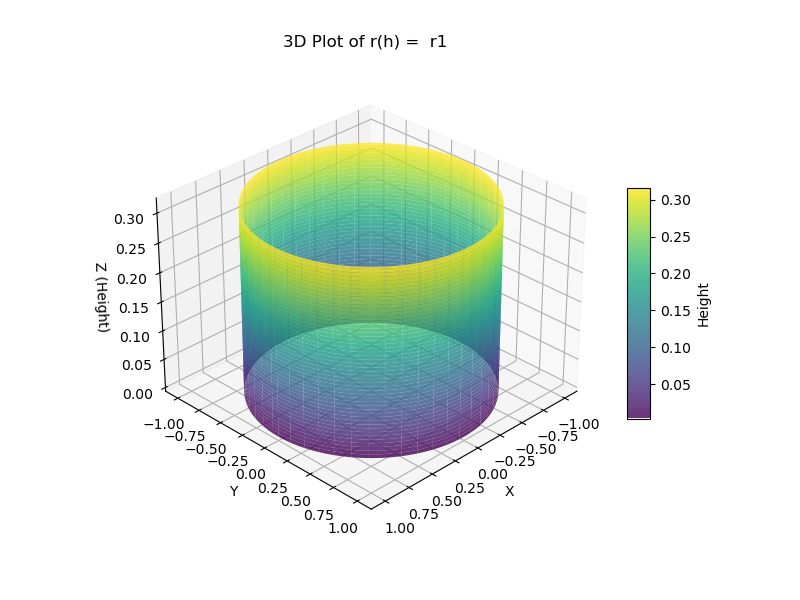
\includegraphics[width=\linewidth]{figures/4_(i) 3D Plot.png}
        \caption{Model (i): Cylinder}
        \label{fig:shape_i}
    \end{subfigure}
    \hfill
    \begin{subfigure}[b]{0.32\textwidth}
        \centering
        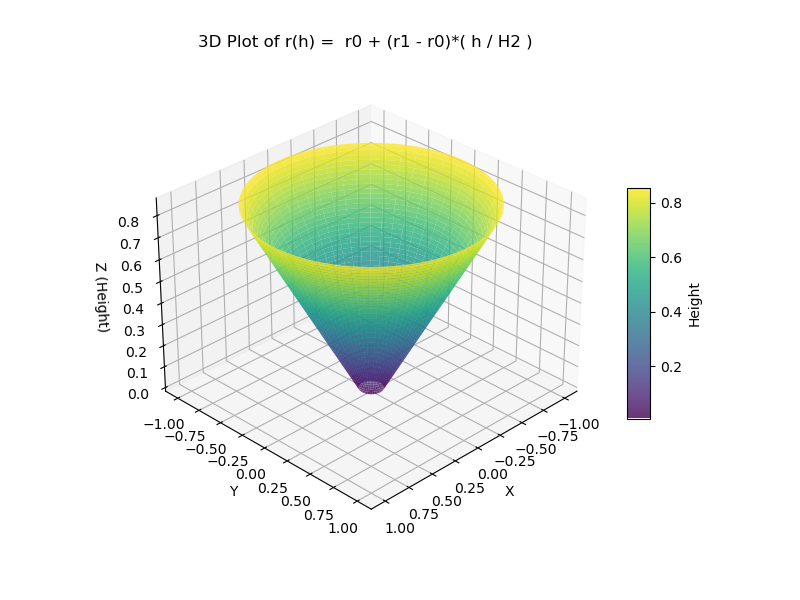
\includegraphics[width=\linewidth]{figures/4_(ii) 3D Plot.png}
        \caption{Model (ii): Linear}
        \label{fig:shape_ii}
    \end{subfigure}
    \hfill
    \begin{subfigure}[b]{0.32\textwidth}
        \centering
        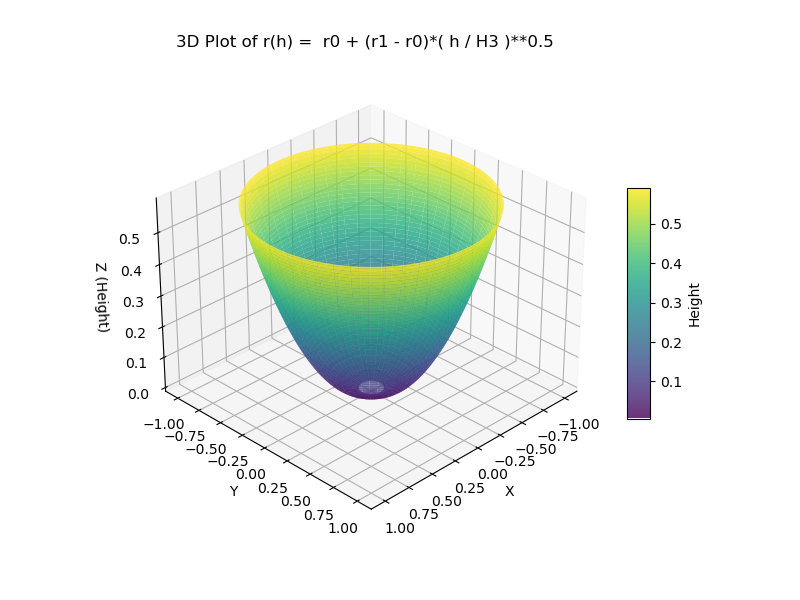
\includegraphics[width=\linewidth]{figures/4_(iii) 3D Plot.png}
        \caption{Model (iii): Square Root}
        \label{fig:shape_iii}
    \end{subfigure}
    
    \vspace{0.5cm}
    
    % Bottom Row: 2 images
    \begin{subfigure}[b]{0.32\textwidth}
        \centering
        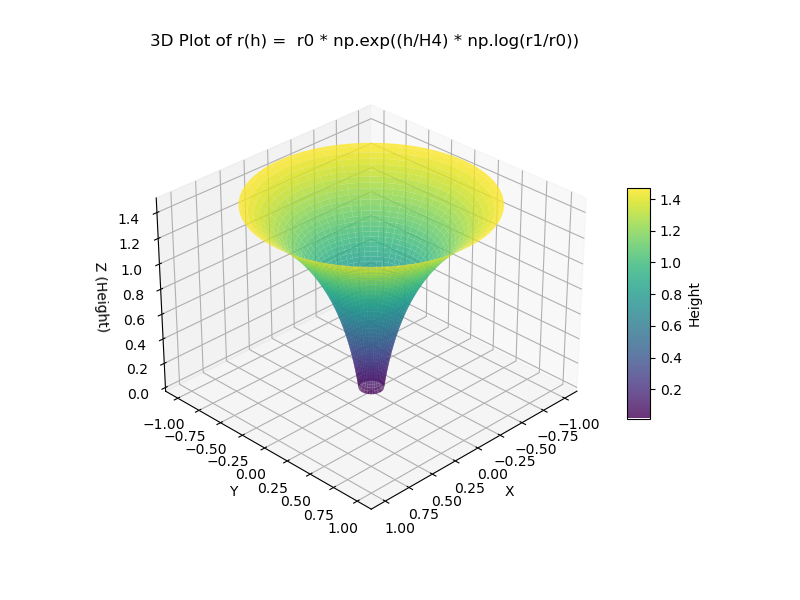
\includegraphics[width=\linewidth]{figures/4_(iv) 3D Plot.png}
        \caption{Model (iv): Exponential}
        \label{fig:shape_iv}
    \end{subfigure}
    \hspace{2cm}
    \begin{subfigure}[b]{0.32\textwidth}
        \centering
        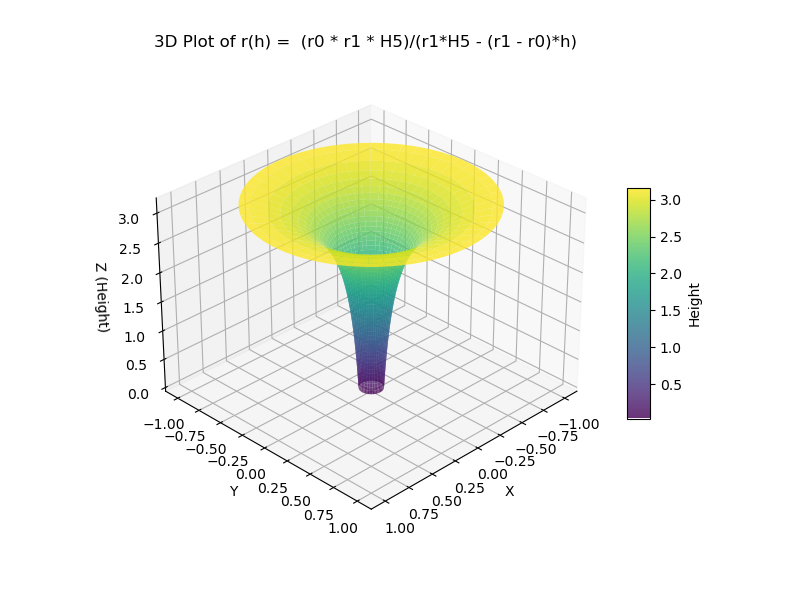
\includegraphics[width=\linewidth]{figures/4_(v) 3D Plot.png}
        \caption{Model (v): Rational}
        \label{fig:shape_v}
    \end{subfigure}
    
    \caption{3D visualization of the five container shapes}
    \label{fig:all_shapes}
\end{figure}

\textbf{Geometric Interpretation:}
The visualization highlights a fundamental geometric trade-off imposed by the fixed volume constraint ($V=1 \text{ ft}^3$). As the container profile shifts from \textbf{convex} (e.g., Cylinder) to \textbf{concave} (e.g., Rational), the fluid distribution changes from ``horizontal" to ``vertical".

Consequently, the Rational Shape (v) achieves an initial height ($H \approx 3.18$ ft) nearly \textbf{10 times greater} than that of the Cylinder ($H \approx 0.32$ ft). By constricting the fluid volume at the base (creating a ``hyperbolic funnel"), Model (v) maximizes the potential energy head, establishing the geometric foundation for flow stability.

\subsection{Numerical Solution of Liquid Height $h(t)$}

\subsubsection{Mathematical Well-Posedness}
Before performing numerical simulations, we establish the theoretical existence of the solution. The governing differential equation derived from Torricelli's Law is:
\begin{equation}
    \frac{dh}{dt} = -\frac{\alpha a \sqrt{2gh}}{\pi \left[r(h)\right]^2} = f(t,h)
\end{equation}

According to the \textbf{Existence and Uniqueness Theorem} , a unique solution exists for $t \ge 0$ provided that $f(t, h)$ and its partial derivative $\frac{\partial f}{\partial h}$ are continuous. 
For our container geometries, as long as the liquid height $h > 0$ and the radius $r(h) \neq 0$, these conditions are strictly satisfied. This guarantees that the physical trajectory we calculate is unique and deterministic.

\subsubsection{Selection of Numerical Method}
While analytical methods such as Picard Iteration (integral-based) or Power Series (derivative-based) are theoretically sound, they face practical limitations for complex geometries like the Rational shape, where the integrals become analytically intractable.

Therefore, we select the Runge-Kutta-Fehlberg method (RK45). It is critical to note that RK45 is essentially a \textbf{numerical optimization of the Taylor Series expansion}. By evaluating the slope at multiple points within a time step, RK45 mimics the accuracy of a 4th-order Taylor series without requiring the complex symbolic differentiation of higher-order derivatives. This provides the ideal balance between theoretical rigor and computational efficiency.

\subsubsection{Algorithm Description}
The solver computes the liquid level $h_{n+1}$ at time $t_{n+1} = t_n + \Delta t$ based on a weighted average of slopes ($k$) calculated at four points within the interval:

\begin{equation}
    h_{n+1} \approx h_n + \frac{\Delta t}{6} (k_1 + 2k_2 + 2k_3 + k_4)
\end{equation}

Where the slopes are determined as:
\begin{align*}
    k_1 &= f(t_n, h_n) \\
    k_2 &= f(t_n + \frac{\Delta t}{2}, h_n + \frac{\Delta t}{2}k_1) \\
    k_3 &= f(t_n + \frac{\Delta t}{2}, h_n + \frac{\Delta t}{2}k_2) \\
    k_4 &= f(t_n + \Delta t, h_n + \Delta t k_3)
\end{align*}

The algorithm automatically adjusts the time step $\Delta t$ to keep the local truncation error below a specified tolerance ($10^{-6}$ in our simulation). We also implemented a continuous event detection mechanism to terminate the integration precisely when $h(t)$ crosses zero, avoiding complex number errors from the square root of negative heights.

\subsubsection{Simulation Results}
The simulation was performed for $t \in [0, 60]$ seconds. The resulting height curves $h(t)$ are shown in Figure \ref{fig:4.4.3_Water Height vs Time}, and the precise emptying times are listed in Table \ref{tab:4.4.3_empty_time}.

\begin{figure}[H]
    \centering
    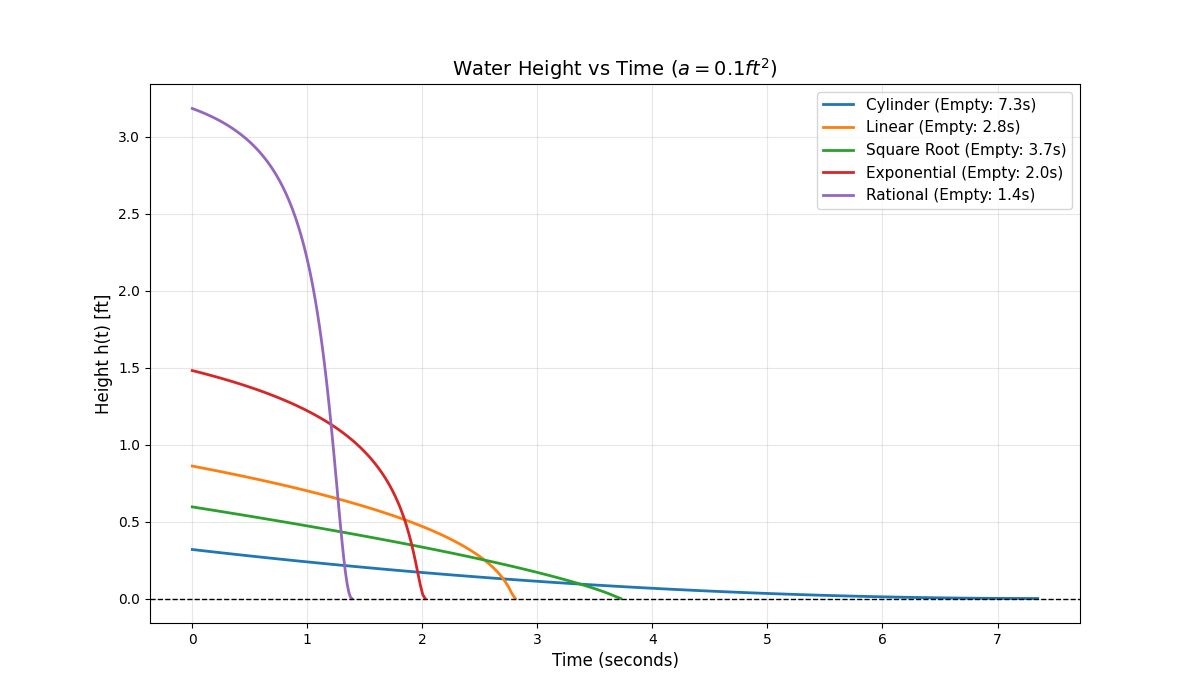
\includegraphics[width=1.0\textwidth]{figures/4.4.3_Water Height vs Time.png}
    \caption{Liquid level $h(t)$ vs. Time for the five containers}
    \label{fig:4.4.3_Water Height vs Time}
\end{figure}



\begin{table}[H]
    \centering
    \caption{Comparison of Initial Heights and Emptying Times}
    \label{tab:4.4.3_empty_time}
    \begin{tabular}{lccc}
    \toprule
    \textbf{Model ID} & \textbf{Shape Description} & \textbf{Initial Height $H$ (ft)} & \textbf{Emptying Time $t_{empty}$ (s)} \\
    \midrule
    i & Cylinder & 0.3183 & 7.3 \\
    ii & Linear & 0.8603 & 2.8 \\
    iii & Square Root & 0.5950 & 3.7 \\
    iv & Exponential & 1.4807 & 2.0 \\
    v & Rational & 3.1831 & 1.4 \\
    \bottomrule
    \end{tabular}
\end{table}

\textbf{Analysis of Emptying Times:}
The simulation results reveal a distinct inverse relationship between the initial height $H$ and the emptying time $t_{empty}$.

\begin{enumerate}
    \item \textbf{Impact of Hydrostatic Head}: The Rational Shape (v) possesses the greatest initial height ($H \approx 3.18$ ft). According to Torricelli's Law, outflow velocity is proportional to the square root of the height ($v \propto \sqrt{h}$). Therefore, the Rational container generates the highest initial driving pressure, forcing the fixed volume of water ($1 \text{ ft}^3$) to evacuate rapidly in just $1.4$ seconds.
    
    \item \textbf{Low Head vs. High Head}: Conversely, the Cylinder (i) has the lowest initial height ($H \approx 0.32$ ft). This results in a weak driving force and a much slower outflow velocity, extending the draining duration to $7.3$ seconds.
    
    \item \textbf{Parameter Context}: It is important to note that the rapid draining across all models (mostly under 5 seconds) is due to the large outlet area parameter ($a=0.1 \text{ ft}^2$) relative to the container volume. While the Rational shape drains the fastest due to high pressure, the \textit{stability} of its flow rate relative to its initial value (analyzed in Section 4.5) remains the key criterion for design optimization.
\end{enumerate}

\subsection{Flow Rate Stability and Design Criteria}

To rigorously evaluate the design, we employ two complementary analytical methods: a theoretical power series expansion to characterize the initial dynamics, and a dimensionless ratio analysis to assess long-term stability.

% --- NEW PART: THE POWER SERIES SOLUTION ---
\subsubsection{Theoretical Analysis of Early-Stage Behavior}
The problem explicitly requests an analysis of the flow rate during the ``early stages" ($t \to 0$). Since the numerical solver (RK45) provides discrete approximations, we derive the exact local Taylor series expansion for the liquid height $h(t)$ to validate the physics. The solution takes the form:
\begin{equation}
    h(t) \approx c_0 + c_1 t + c_2 t^2 + O(t^3)
\end{equation}
Where the coefficients are derived analytically from the governing ODE and the chain rule:
\begin{itemize}
    \item $c_0 = H$: The initial height.
    \item $c_1 = -\frac{\alpha a \sqrt{2gH}}{\pi r(H)^2}$: The initial velocity (negative, indicating drainage).
    \item $c_2 = \frac{1}{2} \frac{d}{dt}(h'(t))|_{t=0}$: The initial acceleration, which depends on the wall slope $r'(H)$.
\end{itemize}

Table \ref{tab:taylor_coeffs} presents the calculated coefficients. 

\begin{table}[H]
    \centering
    \caption{Exact Taylor Series Coefficients for $h(t)$ at $t=0$.}
    \label{tab:taylor_coeffs}
    \begin{tabular}{lccc}
    \toprule
    \textbf{Model} & \textbf{$c_0$ (Height)} & \textbf{$c_1$ (Velocity)} & \textbf{$c_2$ (Acceleration)} \\
    \midrule
    (i) Cylinder & 0.3183 & -0.0865 & 0.0059 \\
    (ii) Linear & 0.8603 & -0.1422 & -0.0153 \\
    (iii) Sq. Root & 0.5950 & -0.1182 & -0.0047 \\
    (iv) Exponential & 1.4807 & -0.1865 & -0.0482 \\
    (v) Rational & 3.1831 & -0.2734 & -0.2055 \\
    \bottomrule
    \end{tabular}
\end{table}

\textbf{Insight:} While the Rational shape (v) has the fastest initial velocity ($c_1 = -0.2734$), it also has the strongest negative acceleration ($c_2 = -0.2055$). This mathematically confirms that the geometry exerts a strong ``braking" force on the flow rate changes immediately after $t=0$.

% --- EXISTING PART: STABILITY METRIC ---
\subsubsection{Definition of Stability Metric $R(t)$}
We define a dimensionless flow rate ratio $R(t)$ to normalize the results:
\begin{equation}
    R(t) = \frac{F_R(t)}{F_R(0)} = \sqrt{\frac{h(t)}{H}}
\end{equation}
The ideal design target is for $R(t)$ to remain close to 1.0.

% --- EXISTING PART: SIMULATION RESULTS ---
\subsubsection{Analysis of Simulation Results}
Figure \ref{fig:4.5_Flow_Rate_Ratio} presents the evolution of $R(t)$ derived from the RK45 simulation.

\begin{figure}[H]
    \centering
    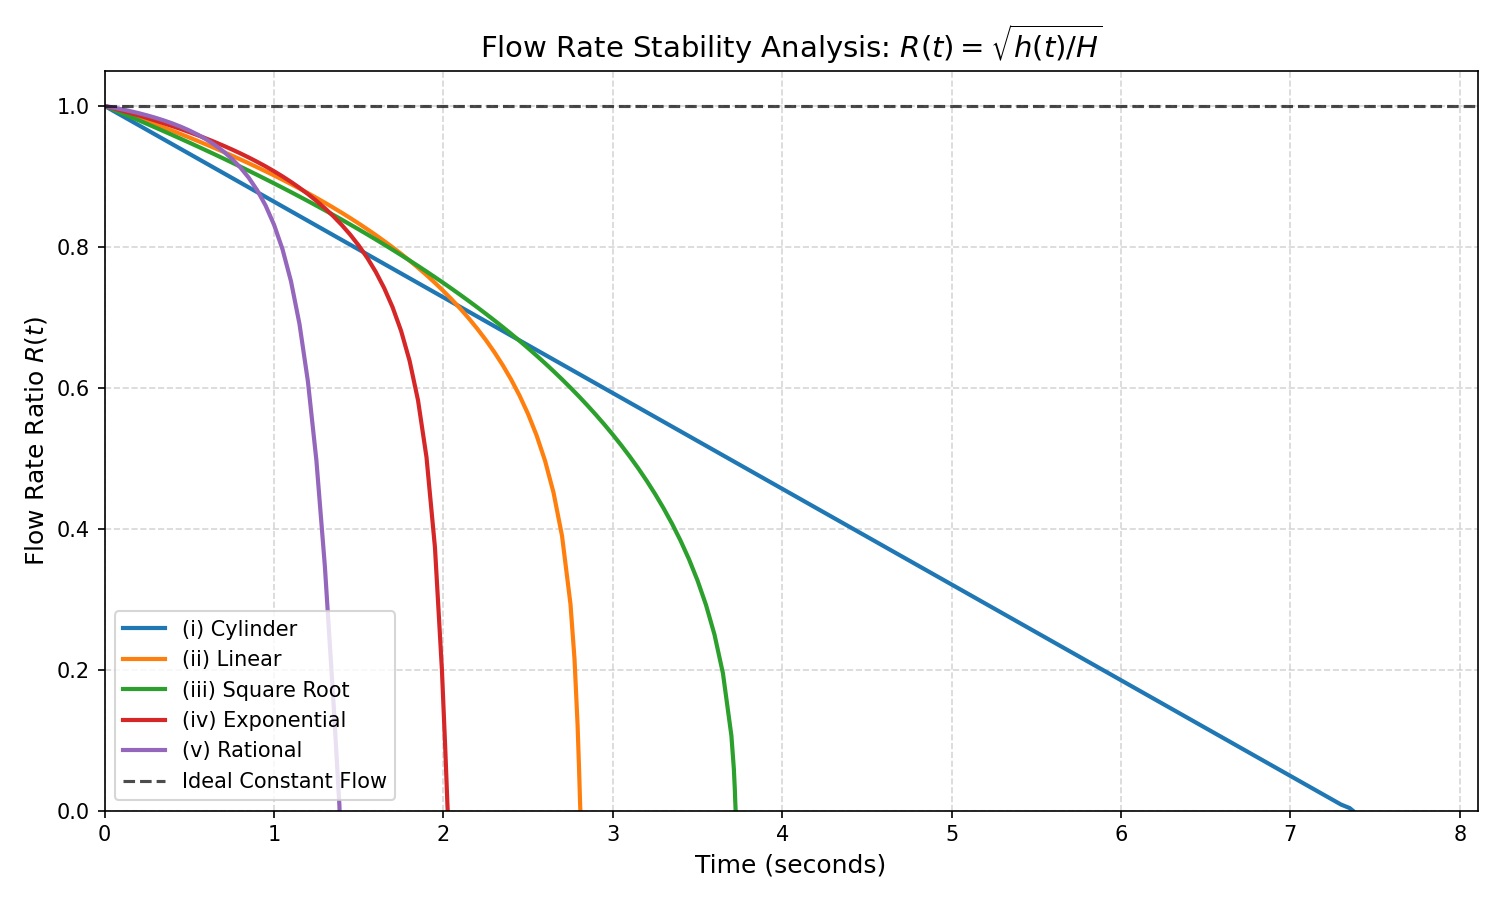
\includegraphics[width=0.9\textwidth]{figures/4.5_Flow Rate Ratio.png}
    \caption{Comparison of the dimensionless flow rate ratio $R(t)$.}
    \label{fig:4.5_Flow_Rate_Ratio}
\end{figure}

% --- EXISTING PART: TAYLOR APPROXIMATION ANALYSIS ---
\textbf{Quantitative Stability Mechanism:}
We observe that the Rational Shape (v) remains closest to $R(t)=1$. To explain this, we approximate $R(t)$ for small height drops $\Delta h$:
\begin{equation} \label{eq:taylor}
    R(t) = \sqrt{1 - \frac{\Delta h}{H}} \approx 1 - \frac{1}{2} \left( \frac{\Delta h}{H} \right)
\end{equation}

Equation \eqref{eq:taylor} demonstrates that the deviation is \textbf{inversely proportional to the initial height} $H$.
\begin{itemize}
    \item \textbf{Model (i) Cylinder}: $H \approx 0.32 \implies$ Error $\propto \frac{1}{0.32} \approx 3.1$.
    \item \textbf{Model (v) Rational}: $H \approx 3.18 \implies$ Error $\propto \frac{1}{3.18} \approx 0.31$.
\end{itemize}

\textbf{Conclusion:} The Rational model reduces flow rate deviation by a factor of $\approx 10$. By geometrically forcing a large $H$, it acts as a hydrostatic buffer.

\subsection{Qualitative Description of the Optimal Container}
The problem asks to sketch the suitable container shape based on these computer experiments. The numerical results confirm that to minimize the variance in flow rate ($\frac{dR}{dt} \approx 0$), the geometric design must satisfy the condition that the relative height change $\frac{dh}{H}$ is minimized.

Therefore, the suitable container should possess the following physical characteristics:
\begin{itemize}
    \item \textbf{Overall Form}: The container must be extremely tall and slender to maximize the initial pressure head $H$.
    \item \textbf{Bottom}: The radius should not increase linearly. Instead, it should remain small near the bottom (to minimize volume storage in the low-pressure zone) and flare out rapidly at the top.
    \item \textbf{Top}: The resulting shape resembles a \textbf{trumpet} or an elongated \textbf{funnel} (specifically, a hyperbolic funnel).
\end{itemize}

This geometry ensures that the majority of the liquid volume is stored at a high potential energy state. As liquid drains, the drop in height is initially small relative to the total head, maintaining a nearly constant driving force.

\section{Problem 2: Optimal Shape Based on Potential Energy}

\subsection{Theoretical Derivation: The Iso-Potential Condition}
The problem introduces a physical criterion for the ideal container: it must consist of fluid parcels ``all possessing the same amount of potential energy.'' 

We analyze this constraint using fundamental physics:
\begin{enumerate}
    \item \textbf{Potential Energy Definition}: The gravitational potential energy of a fluid mass $m$ is $E_p = mgh$.
    \item \textbf{Geometric Implication}: For every parcel to possess the exact same energy $E_p$, every parcel must reside at the exact same vertical elevation $h$.
    \item \textbf{The Limit Case}: Geometrically, the only shape where a finite volume $V$ exists entirely at a single elevation $H$ is the limit case of a cylinder with infinite cross-sectional area $A \to \infty$ and infinitesimal height $H \to 0$ (a ``flat sheet'' of water).
\end{enumerate}

\textbf{Foreshadowing the Flow Behavior:}
Consider a cylinder of fixed volume $V=1$. Its cross-sectional area is constrained by $A = V/H$.
The rate of change of the flow ratio $R(t)$ at $t=0$ is governed by:
\begin{equation}
    \frac{dR}{dt} \propto \frac{1}{A \sqrt{H}} = \frac{1}{(V/H)\sqrt{H}} = \frac{\sqrt{H}}{V}
\end{equation}
\textbf{Prediction:} This derivation predicts that the instability (decay rate) is proportional to $\sqrt{H}$. Therefore, as we reduce the initial height $H$ (and consequently widen the cylinder), the slope of $R(t)$ should approach zero, yielding a perfectly stable flow.

\subsection{Numerical Verification}
To validate this theoretical prediction, we conducted a computational experiment simulating cylindrical containers of fixed volume ($V=1 \text{ ft}^3$) across varying orders of magnitude for initial height, ranging from $H=10$ ft (Tall/Narrow) to $H=10^{-6}$ ft (Flat/Wide).

The simulation results are visualized in Figure \ref{fig:5.2_Flow Rate Stability}.

\begin{figure}[H]
    \centering
    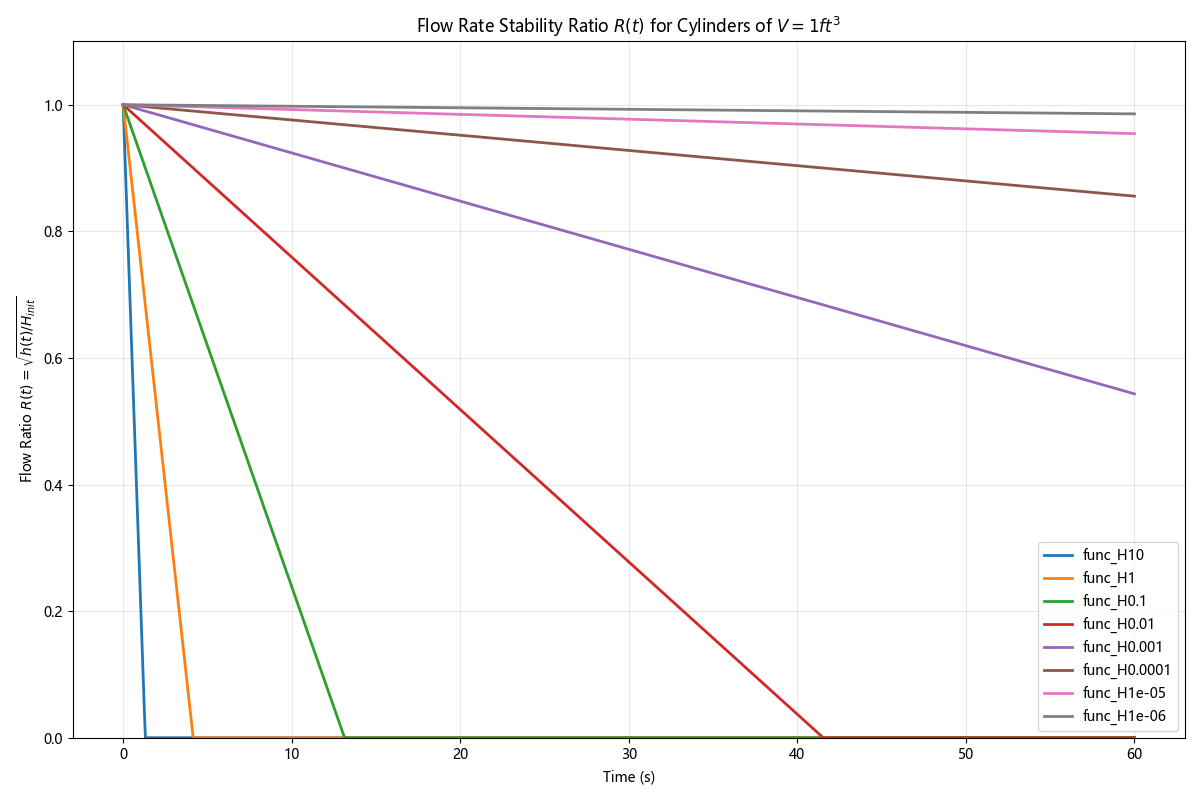
\includegraphics[width=1.0\textwidth]{figures/5.2_Flow Rate Stability.png}
    \caption{Flow Rate Stability Ratio $R(t)$ for Cylinders of fixed volume ($V=1$)}
    \label{fig:5.2_Flow Rate Stability}
\end{figure}

\subsection{Analysis of Draining Duration}

The simulation results provide a stark contrast in the temporal dynamics of the containers, confirming the inverse relationship between initial height and flow duration.

\begin{enumerate}
    \item \textbf{The Unstable Regime ($H \ge 1$)}: 
    For tall cylinders, the high initial potential energy is rapidly converted into kinetic energy. The draining process is extremely transient, with the container emptying in a few seconds. This confirms that high-aspect-ratio cylinders are unsuitable for maintaining a steady state over the required 60-second interval.

    \item \textbf{The Quasi-Stable Regime ($H \le 0.01$)}: 
    As the initial height decreases by orders of magnitude, the draining duration increases exponentially. For $H=0.01$ ft, the duration extends significantly, approaching the experiment's time horizon. Most importantly, for the approximation of the ideal shape ($H \le 0.001$ ft), the container retains the vast majority of its volume throughout the entire observation window.
    
    \item \textbf{Convergence to Infinity}: 
    Mathematically, the emptying time $t_{empty}$ scales with $A/\sqrt{a}$. Since $A \propto 1/H$, it follows that $t_{empty} \propto 1/H$. As $H \to 0$, the emptying time diverges to infinity ($t_{empty} \to \infty$). This asymptotic behavior confirms that the limit case is a reservoir that effectively never drains, thereby maintaining a constant pressure head and a perfectly stable flow rate ($R=1$) indefinitely.
\end{enumerate}

\subsection{Discussion and Conclusion}

The numerical results in Figure \ref{fig:5.2_Flow Rate Stability} strongly corroborate the theoretical derivation. We draw three critical mathematical conclusions:

\subsubsection{Proof of Cylindrical Linearity}
A striking feature of Figure \ref{fig:5.2_Flow Rate Stability} is that all curves are perfectly straight lines. We can prove this analytically.
For a cylinder, $A(h)$ is constant. The ODE is:
\begin{equation}
    \frac{dh}{dt} = -k \sqrt{h} \quad \text{where } k = \frac{\alpha a \sqrt{2g}}{A}
\end{equation}
To find the flow ratio $R(t) = \sqrt{h(t)/H}$, we differentiate $R$ with respect to time using the chain rule:
\begin{equation}
    \frac{dR}{dt} = \frac{d}{dt}\left( \frac{h^{1/2}}{H^{1/2}} \right) = \frac{1}{2\sqrt{hH}} \frac{dh}{dt} = \frac{1}{2\sqrt{hH}} (-k\sqrt{h}) = -\frac{k}{2\sqrt{H}} = \text{Constant}
\end{equation}
Since the derivative $\frac{dR}{dt}$ is constant, $R(t)$ must be linear. This confirms that our simulation correctly models cylindrical physics.

\subsubsection{Resolution of the Geometric Paradox}
It is essential to reconcile the results of Problem 1 (which favored the tallest shape) with Problem 2 (which favors the flattest shape).
\begin{itemize}
    \item \textbf{Problem 1 (Fixed Radius Constraint)}: The top radius was locked at $r_1 = 1$. With a fixed area, the only way to minimize the relative drop $\Delta h / H$ was to maximize $H$. Thus, the ``Tall" Rational shape won.
    \item \textbf{Problem 2 (Fixed Volume Constraint)}: The geometry was unconstrained. Since stability scales with $A\sqrt{H}$ (or $\frac{\sqrt{H}}{V}$), and $A$ and $H$ are inversely related ($A=V/H$), increasing $A$ (widening) is mathematically far more potent than increasing $H$. Thus, the ``Flat" Cylinder wins.
\end{itemize}

\subsubsection{Final Design Recommendation}
Based on potential energy considerations, the Ideal Shape is an Infinite Reservoir (a cylinder with maximal radius and minimal height). This geometry creates a Constant Head system where the kinetic energy loss from draining is negligible compared to the total potential energy stored in the vast surface area, maintaining $R(t) \approx 1$ indefinitely.

% ========================================================
% GENERAL PROJECT CONCLUSION
% ========================================================
\section{General Project Conclusion and Design Recommendations}

This project explored the design of a constant-flow drip dispenser through the lens of differential equations, numerical simulation, and physical theory. The investigation yielded two distinct, yet mathematically consistent, conclusions based on the constraints applied.

\subsection{Summary of Findings}
\begin{enumerate}
    \item \textbf{Constrained Optimization (The Laboratory Case)}: 
    When the container's top radius is constrained (e.g., $r=1$ ft), the optimal strategy is to maximize the vertical aspect ratio. 
    \begin{itemize}
        \item \textbf{Mathematical Proof}: The Taylor series expansion identified a ``hydraulic braking" term ($c_2 \approx -0.20$) in the Rational shape that is absent in cylindrical shapes.
        \item \textbf{Result}: The Rational (Hyperbolic Funnel) shape creates the highest possible pressure head $H \approx 3.18$ ft, minimizing the relative head loss $\frac{\Delta h}{H}$.
    \end{itemize}

    \item \textbf{Unconstrained Optimization (The Physics Case)}:
    When spatial constraints are removed, the fundamental physics dictates that stability is driven by the conservation of potential energy across fluid parcels.
    \begin{itemize}
        \item \textbf{Mathematical Proof}: The scaling law derivation confirmed that instability scales with $\sqrt{H}$.
        \item \textbf{Result}: The ideal shape is the limit case of $H \to 0$ and $A \to \infty$ (an Infinite Reservoir).
    \end{itemize}
\end{enumerate}

\subsection{Resolution of the Geometric Paradox}
The study resolves the apparent contradiction between \enquote{Tallest is Bests} (Problem 1) and \enquote{Shortest is Best}  (Problem 2). 
The flow stability is governed by the ratio of Volume to Height, specifically the term $A\sqrt{H}$. 
\begin{itemize}
    \item In Problem 1, $A$ was fixed at the top, so we had to increase $H$ to gain stability (a second-order benefit).
    \item In Problem 2, we could increase $A$ directly. Since $A \propto 1/H$, increasing $A$ reduces stability decay much faster than increasing $H$ helps.
\end{itemize}

\subsection{Final Recommendation}
For a practical laboratory setting where bench space (width) is limited but vertical space is available, the Rational Shape (Model v) is the optimal design. It approximates a \enquote{Constant Head} device by stacking the fluid vertically, ensuring that the driving pressure remains nearly constant during the critical early stages of the experiment.







\newpage
\appendix
\renewcommand{\thesection}{A} % Force Appendix to be Section A

\section{Appendix: Computational Source Code}

% --- Professional Code Style Definition ---


\definecolor{codegreen}{rgb}{0,0.6,0}
\definecolor{codegray}{rgb}{0.5,0.5,0.5}
\definecolor{codepurple}{rgb}{0.58,0,0.82}
\definecolor{backcolour}{rgb}{0.98,0.98,0.98}

\lstdefinestyle{academicStyle}{
    backgroundcolor=\color{backcolour},   
    commentstyle=\color{codegreen}\itshape,
    keywordstyle=\color{blue}\bfseries,
    numberstyle=\tiny\color{codegray},
    stringstyle=\color{codepurple},
    basicstyle=\ttfamily\footnotesize, % Monospaced font
    breakatwhitespace=false,         
    breaklines=true,                 
    captionpos=t,                      % Caption at the top
    keepspaces=true,                 
    numbers=left,                      % Line numbers
    numbersep=5pt,                  
    showspaces=false,                
    showstringspaces=false,
    showtabs=false,                  
    tabsize=4,
    frame=tb,                          % Top and Bottom lines only (Professional look)
    framerule=0.5pt,
    rulecolor=\color{black},
    language=Python
}

\lstset{style=academicStyle}

\subsection*{1. Calculation of $H$ and 3D Plotting}

\begin{lstlisting}
import sympy as sp
import numpy as np
import matplotlib.pyplot as plt
import inspect

r0 = sp.symbols('r0', positive=True)
r1 = sp.symbols('r1', positive=True)
alpha = sp.symbols('alpha', positive=True)
a = sp.symbols('a', positive=True)
h = sp.symbols('h')
H = sp.symbols('H', positive=True)

func1 = r1
func2 = r0 + (r1 - r0)*( h / H )
func3 = r0 + (r1 - r0)*sp.sqrt(( h / H ))
func4 = r0 * sp.exp((h/H) * sp.log(r1/r0))
func5 = (r0 * r1 * H)/(r1*H - (r1 - r0)*h)

def calculate_H(func):
    volume_integral = sp.integrate(sp.pi * func**2, (h, 0, H))
    volume_eq = sp.Eq(volume_integral, 1)
    H_solution = sp.solve(volume_eq, H)
    return H_solution

print(f"r1_H: {calculate_H(func1)}")
print(f"r2_H: {calculate_H(func2)}")
print(f"r3_H: {calculate_H(func3)}")
print(f"r4_H: {calculate_H(func4)}")
print(f"r5_H: {calculate_H(func5)}")

r0 = 0.1
r1 = 1
alpha = 0.6
a = 0.1

H1 = 1 / (np.pi * r1**2)
H2 = 3 / (np.pi * (r0**2 + r0*r1 + r1**2))
H3 = 6 / (np.pi*(r0**2 + 2*r0*r1 + 3*r1**2))
H4 = np.log((r0/r1)**(2/np.pi))/(r0**2 - r1**2)
H5 = 1/(np.pi*r0*r1)

func1 = lambda h: r1
func2 = lambda h: r0 + (r1 - r0)*( h / H2 )
func3 = lambda h: r0 + (r1 - r0)*( h / H3 )**0.5
func4 = lambda h: r0 * np.exp((h/H4) * np.log(r1/r0))
func5 = lambda h: (r0 * r1 * H5)/(r1*H5 - (r1 - r0)*h)

def plot_container(func, H, save_path=None):
    theta = np.linspace(0, 2 * np.pi, 100)
    h = np.linspace(0, H, 100)

    theta_grid, h_grid = np.meshgrid(theta, h)

    x = func(h_grid) * np.cos(theta_grid)
    y = func(h_grid) * np.sin(theta_grid)
    z = h_grid

    fig = plt.figure(figsize=(8, 6))
    ax = fig.add_subplot(111, projection='3d')

    ax.view_init(elev=30, azim=45)

    surface = ax.plot_surface(
        x, y, z,
        cmap='viridis',
        alpha=0.8,
        edgecolor='none'
    )

    ax.set_xlabel('X')
    ax.set_ylabel('Y')
    ax.set_zlabel('Z (Height)')
    ax.set_title(f'3D Plot of r(h) = {inspect.getsource(func)[17:]}')

    fig.colorbar(surface, ax=ax, shrink=0.5, aspect=10, label='Height')

    if save_path:
        plt.savefig(save_path)

    plt.show()

if __name__ == "__main__":
    plot_container(func1, H1, 'func1.png')
    plot_container(func2, H2, 'func2.png')
    plot_container(func3, H3, 'func3.png')
    plot_container(func4, H4, 'func4.png')
    plot_container(func5, H5, 'func5.png')
\end{lstlisting}

\subsection*{2. RK45 Numerical Solver implementation}

\begin{lstlisting}
import numpy as np
import matplotlib.pyplot as plt
from scipy.integrate import solve_ivp
from scipy.optimize import brentq
from scipy.integrate import quad

g = 32.2
a = 0.1
alpha = 0.6
r0 = 0.1
r1 = 1.0 
target_vol = 1.0

C = (alpha * a * np.sqrt(2 * g)) / np.pi 

def get_radius(h, H, shape_type):
    if h < 0: h = 0
    
    if shape_type == 'Cylinder':
        return r1
    elif shape_type == 'Linear':
        return r0 + (r1 - r0) * (h/H)
    elif shape_type == 'Square Root':
        return r0 + (r1 - r0) * np.sqrt(h/H)
    elif shape_type == 'Exponential':
        return r0 * np.exp((h/H) * np.log(r1/r0))
    elif shape_type == 'Rational':
        denom = r1 * H - (r1 - r0) * h
        if denom <= 0: return r1
        return (r0 * r1 * H) / denom
    return r1

def volume_mismatch(H, shape_type):
    if H <= 0: return -1.0
    integrand = lambda h: np.pi * get_radius(h, H, shape_type)**2
    vol, _ = quad(integrand, 0, H)
    return vol - target_vol

shapes = ['Cylinder', 'Linear', 'Square Root', 'Exponential', 'Rational']
initial_heights = {}

print("Initial Heights (H):")
for shape in shapes:
    H_sol = brentq(volume_mismatch, 0.01, 20.0, args=(shape,))
    initial_heights[shape] = H_sol
    print(f"  {shape}: {H_sol:.4f} ft")

def drain_ode(t, h, H, shape_type):
    if h <= 0: return 0
    r = get_radius(h, H, shape_type)
    dhdt = -C * np.sqrt(h) / (r**2)
    return dhdt

def empty_tank(t, h, H, shape_type):
    return h
empty_tank.terminal = True
empty_tank.direction = -1

t_span = (0, 60)
results = {}

print("\nTime to Empty:")
plt.figure(figsize=(12, 7))

for shape in shapes:
    H = initial_heights[shape]

    sol = solve_ivp(
        drain_ode, 
        t_span, 
        [H], 
        args=(H, shape), 
        events=empty_tank,
        max_step=0.1,
        dense_output=True
    )
    
    results[shape] = sol
    t_empty = sol.t[-1] if sol.status == 1 else 60.0
    print(f"  {shape}: {t_empty:.2f} s")

    t_plot = np.linspace(0, t_empty, 100)
    h_plot = sol.sol(t_plot)[0]
    plt.plot(t_plot, h_plot, label=f"{shape} (Empty: {t_empty:.1f}s)", linewidth=2)

plt.title(f"Water Height vs Time ($a={a} ft^2$)", fontsize=14)
plt.xlabel("Time (seconds)", fontsize=12)
plt.ylabel("Height h(t) [ft]", fontsize=12)
plt.axhline(0, color='k', linestyle='--', linewidth=1)
plt.grid(True, alpha=0.3)
plt.legend(fontsize=11)
plt.show()
\end{lstlisting}

\subsection*{3. Calculation of Taylor Series Coefficients}

\begin{lstlisting}
import numpy as np

g = 32.2
a = 0.1
alpha = 0.6
r0, r1 = 0.1, 1.0
C = (alpha * a * np.sqrt(2 * g)) / np.pi

def get_H_and_Coeffs(shape_name):
    if 'Cylinder' in shape_name: H = 0.3183
    elif 'Linear' in shape_name: H = 0.8603
    elif 'Square' in shape_name: H = 0.5950
    elif 'Exponential' in shape_name: H = 1.4807
    elif 'Rational' in shape_name: H = 3.1831

    r_H = r1 
    
    if 'Cylinder' in shape_name:
        dr_dh = 0
    elif 'Linear' in shape_name: 
        dr_dh = (r1 - r0) / H
    elif 'Square' in shape_name:
        dr_dh = (r1 - r0) / (2 * H)
    elif 'Exponential' in shape_name:
        dr_dh = r1 * np.log(r1/r0) / H
    elif 'Rational' in shape_name:
        dr_dh = (r1 * (r1 - r0)) / (r0 * H)
    c0 = H
    c1 = -C * np.sqrt(H) / (r_H**2)
    accel_term = (C**2 / 2) * (1 - 4 * H * dr_dh / r_H)
    c2 = accel_term / 2
    
    return c0, c1, c2

shapes = ['Cylinder', 'Linear', 'Square Root', 'Exponential', 'Rational']
print(f"{'Model':<15} | {'c0 (H)':<10} | {'c1 (Vel)':<10} | {'c2 (Accel)':<10}")
print("-" * 55)
for s in shapes:
    c0, c1, c2 = get_H_and_Coeffs(s)
    print(f"{s:<15} | {c0:<10.4f} | {c1:<10.4f} | {c2:<10.4f}")
\end{lstlisting}

\subsection*{4. Plotting Flow Rate Ratio $R(t)$ for 5 Models}

\begin{lstlisting}
import numpy as np
import matplotlib.pyplot as plt
from scipy.integrate import solve_ivp, quad
from scipy.optimize import brentq

g = 32.2
a = 0.1
alpha = 0.6
target_vol = 1.0
r0 = 0.1
r1 = 1.0

C_ode = (alpha * a * np.sqrt(2 * g)) / np.pi 

def get_radius(h, H, shape_name):
    if h < 0: h = 0
    
    if shape_name == '(i) Cylinder':
        return r1
    elif shape_name == '(ii) Linear':
        return r0 + (r1 - r0) * (h / H)
    elif shape_name == '(iii) Square Root':
        return r0 + (r1 - r0) * np.sqrt(h / H)
    elif shape_name == '(iv) Exponential':
        return r0 * np.exp((h / H) * np.log(r1 / r0))
    elif shape_name == '(v) Rational':
        denom = r1 * H - (r1 - r0) * h
        if denom <= 1e-9: return r1
        return (r0 * r1 * H) / denom
    return r1

def solve_H_for_shape(shape_name):
    def volume_error(H_guess):
        if H_guess <= 0: return -target_vol
        integrand = lambda h: np.pi * (get_radius(h, H_guess, shape_name)**2)
        vol, _ = quad(integrand, 0, H_guess)
        return vol - target_vol
    
    return brentq(volume_error, 0.05, 20.0)

def drain_ode(t, h, H, shape_name):
    if h <= 0: return 0
    r = get_radius(h, H, shape_name)
    return -C_ode * np.sqrt(h) / (r**2)

def empty_event(t, h, H, shape_name):
    return h
empty_event.terminal = True
empty_event.direction = -1

shape_list = [
    '(i) Cylinder', 
    '(ii) Linear', 
    '(iii) Square Root', 
    '(iv) Exponential', 
    '(v) Rational'
]

plt.figure(figsize=(10, 6), dpi=150)

max_time = 0

for shape in shape_list:
    H_start = solve_H_for_shape(shape)

    sol = solve_ivp(
        drain_ode, 
        (0, 60), 
        [H_start], 
        args=(H_start, shape), 
        events=empty_event,
        dense_output=True,
        max_step=0.05 
    )

    t_vals = sol.t
    h_vals = sol.y[0]
    R_vals = np.sqrt(np.maximum(h_vals, 0) / H_start)

    plt.plot(t_vals, R_vals, linewidth=2, label=shape)
    
    if t_vals[-1] > max_time: max_time = t_vals[-1]

plt.axhline(y=1.0, color='black', linestyle='--', linewidth=1.5, alpha=0.7, label='Ideal Constant Flow')

plt.title(r'Flow Rate Stability Analysis: $R(t) = \sqrt{h(t)/H}$', fontsize=14)
plt.xlabel('Time (seconds)', fontsize=12)
plt.ylabel(r'Flow Rate Ratio $R(t)$', fontsize=12)
plt.xlim(0, max_time * 1.1)
plt.ylim(0, 1.05)
plt.grid(True, which='both', linestyle='--', alpha=0.5)
plt.legend(loc='lower left', fontsize=10, frameon=True)

plt.tight_layout()
plt.savefig('fig_flow_rate.png') 
plt.show()
\end{lstlisting}

\subsection*{5. Simulation of Ideal Shape Limit (Problem 2)}

\begin{lstlisting}
import numpy as np
from scipy.integrate import solve_ivp
import matplotlib.pyplot as plt

plt.rcParams['font.sans-serif'] = ['Arial']

r0 = 0.1
r1 = 1
alpha = 0.6
a = 0.1
g = 32.2

def func(h):
    r1 = 1 / np.sqrt(np.pi * h)
    def sep(h):
        return r1 * np.ones_like(h)
    return sep

def ode_func(t, h, r_func):
    h = np.maximum(h, 1e-10)

    r = r_func(h)
    A = np.pi * r ** 2

    dhdt = -alpha * a * np.sqrt(2 * g * h) / A

    return dhdt

t_span = (0, 60)
t_eval = np.linspace(0, 60, 1000)

results = {}

H = [10,1,0.1,1e-2,1e-3,1e-4,1e-5,1e-6]
r_funcs = [func(h) for h in H]
func_names = [f'func_H{i}' for i in H]

for i, (r_func, name, H) in enumerate(zip(r_funcs, func_names, H), 1):
    print(f"Solving function {i}: {name}")

    sol = solve_ivp(
        lambda t, h: ode_func(t, h, r_func),
        t_span,
        [H],
        t_eval=t_eval,
        method='RK45',
        rtol=1e-8,
        atol=1e-10
    )

    results[name] = {
        't': sol.t,
        'h': sol.y[0],
        'R': alpha * a * np.sqrt(np.maximum(2 * g * sol.y[0], 0)),
        'empty_time': None
    }

    empty_idx = np.where(sol.y[0] <= 0)[0]
    if len(empty_idx) > 0:
        empty_time = sol.t[empty_idx[0]]
        results[name]['empty_time'] = empty_time
        print(f"  Tank empties at t = {empty_time:.2f} seconds")
    else:
        print(f"  Tank not empty within 60 seconds, final height: {sol.y[0][-1]:.10f} ft")

plt.figure(figsize=(12, 8))
for name, data in results.items():
    plt.plot(data['t'], data['R'] / data['R'][0], linewidth=2, label=name)

plt.xlabel('Time (s)')
plt.ylabel(r'Flow Ratio $R(t) = \sqrt{h(t)/H_{init}}$')
plt.title(r'Flow Rate Stability Ratio $R(t)$ for Cylinders of $V=1 ft^3$')
plt.legend()
plt.grid(True, alpha=0.3)
plt.ylim(0, 1.1)
plt.tight_layout()
plt.savefig('R(t).png')
plt.show()
\end{lstlisting}

\end{document}